\documentclass[conference]{IEEEtran}
% Complete paper (25 Nov 2026). Layout and preamble from paper/main.tex (IEEEtran conference, two columns).
% Every number is generated from results/ and runs/ by paper/make_paper_tables.py or quoted from results/*.csv;
% paper/check_numbers.py verifies that each decimal in this file appears in a results file or generated table.
% Compile with pdfLaTeX (Overleaf: upload the paper/ folder and set Paper.tex as the main document).
\usepackage[T1]{fontenc}
\usepackage[utf8]{inputenc}
\usepackage{cite}
\usepackage{amsmath,amssymb}
\usepackage{graphicx}
\usepackage{booktabs}
\usepackage{multirow}
\usepackage{xcolor}
\usepackage{url}
\usepackage[hidelinks]{hyperref}
\graphicspath{{figs/}}
\DeclareMathOperator*{\argmax}{arg\,max}

\begin{document}

\title{Recipe-Supervised Concepts for Robust and Explainable Deepfake Detection: A Leak-Free Study}

\author{
\IEEEauthorblockN{Charan L, Deepak S N, Samrudh N Shindhe, Samarth Gowda G M, and Jyothi R}
\IEEEauthorblockA{Department of Computer Science and Engineering, PES University, Bengaluru, India\\
\{email\} \quad Corresponding author: Jyothi R, \{email\}}
}

\maketitle

\begin{abstract}
Face-swap detectors trained on FaceForensics++ (FF++) lose accuracy on unseen datasets and compressed video, and
their heatmap explanations are rarely tested for faithfulness. We train a detector whose logit is a weighted sum of
ten named forgery concepts plus a penalised residual; the concept labels are the parameters of the self-blending
recipe that creates each training fake, so they need no annotation. The backbone is CLIP ViT-L/14 with LoRA, fused
with an 8$\times$8 block-DCT branch. Under source-video-disjoint FF++ splits, validation-only model
selection and three seeds per model, the detector reaches a cross-dataset video AUC of 0.914 (DFD and the official
Celeb-DF test list) against 0.854 for Swin-B; CLIP with LoRA alone reaches 0.906, and the difference to it is not
statistically significant (95\% CI [$-$0.007, +0.024]). A step-by-step ablation separates the effects. Training on
self-blends produces most of the robustness and calibration gains (AUC at JPEG quality 30: 0.789 to 0.898;
Celeb-DF calibration error: 0.527 to 0.069). The concept bottleneck adds a small, statistically significant AUC gain
(+0.009 over its parent; +0.016 against an otherwise identical linear head) and an inspectable decision: removing
the residual leaves AUC unchanged, and restoring forged patches to their real pixels in the order given by the region
concept lowers the fake probability as fast as the true blend mask does (area 0.281 vs.\ 0.270; random order
0.663). Single-frame H.264 training raises AUC at CRF~40 from 0.644 to 0.688. A 4.71\,M-parameter distilled
student runs at 4.2\,ms per face on a CPU but reaches only 0.804.
\end{abstract}

\begin{IEEEkeywords}
deepfake detection, concept bottleneck, self-blended images, CLIP, interventions, explanation faithfulness,
knowledge distillation
\end{IEEEkeywords}

% =====================================================================================================
\section{Introduction}

Detectors of face manipulation are usually trained on FaceForensics++ (FF++)~\cite{ffpp} and evaluated on datasets
they never saw, most often Google's DeepFakeDetection (DFD)~\cite{dfd} and Celeb-DF~\cite{celebdf}. In-domain video
AUC is close to 1.0 for most modern backbones, so the cross-dataset numbers decide the comparison, and
DeepfakeBench~\cite{deepfakebench} and DF40~\cite{df40} re-evaluate detectors under one protocol because published
numbers come from different splits, frame samples and training sets. Two further requirements come from use.
Uploaded video is re-encoded with JPEG or H.264, which removes high-frequency image content. A verdict also needs a
reason that a reviewer can check; the usual reasons, Grad-CAM~\cite{gradcam} heatmaps or attention
rollout~\cite{rollout}, are computed after the decision, and their faithfulness has to be measured
separately~\cite{tsigos}.

This paper studies a detector built around one design decision: the final logit is computed from ten named
concepts that describe how a face was blended, and the labels for those concepts come from the procedure that
generates the training fakes. Self-blended images (SBI)~\cite{sbi} are pseudo-fakes made by blending a face with a
transformed copy of itself. Our SBI engine records every random choice it makes (blend ratio, colour shift, blur or
sharpening, resampling, affine shift, blended region and mask warping) and turns these choices into a ten-dimensional
target. The concept head therefore receives dense supervision at no labelling cost, and because the decision layer
is linear in the concept activations, switching a concept off has an exact, computable effect on the logit.

The contributions are as follows.
\begin{enumerate}
\item A leak-free evaluation protocol with paired bootstrap statistics over three seeds, and a measurement of what a
random video split did to an earlier checkpoint of this project (Section~\ref{sec:protocol}).
\item A concept-bottleneck detector on CLIP ViT-L/14 with LoRA and a block-DCT branch, supervised by the SBI recipe,
and an ablation in which each addition is compared with its parent model on the same resampled videos
(Sections~\ref{sec:method} and~\ref{sec:results}).
\item An interventional analysis of the trained decision: exact concept switch-off effects on real test videos, a
decomposition into concept and residual paths, and a counterfactual restoration test that replaces forged patches
with the known real pixels (Section~\ref{sec:interv}).
\item Robustness, calibration and distillation results, including single-frame H.264 training and a 65$\times$
smaller student, with all negative outcomes reported.
\end{enumerate}
We train on a reduced FF++ c23 subset (Section~\ref{sec:data}). Published methods train on more data under other
protocols, so we make no state-of-the-art claim; all comparisons are among models trained by us on identical data.

% =====================================================================================================
\section{Related Work}\label{sec:related}

\textbf{Datasets and protocol.} FF++~\cite{ffpp} provides 1,000 YouTube videos and their manipulations;
Celeb-DF~\cite{celebdf} contains face swaps of celebrities with fewer visible artefacts; DFDC~\cite{dfdc} is a large
challenge set. DeepfakeBench~\cite{deepfakebench} reimplements detectors under one training and evaluation code
base and evaluation protocol. DF40~\cite{df40} extends the evaluation to 40 generation methods.

\textbf{Synthetic training fakes.} Face X-ray~\cite{facexray} trains on faces blended from two identities and
predicts the blending boundary. SBI~\cite{sbi} blends a face with a colour- and frequency-transformed copy of the same
face, so the fake contains blending artefacts but no identity change; an EfficientNet-B4~\cite{efficientnet} trained
on real faces and their self-blends generalises well to Celeb-DF. We reuse the SBI construction and keep its random
parameters as labels.

\textbf{Foundation-model detectors.} UnivFD~\cite{univfd} trains a linear probe on frozen CLIP~\cite{clip} features
and generalises across image generators. Forensics Adapter~\cite{fa} adds a trainable adapter next to a frozen CLIP
encoder for face forgery; Effort~\cite{effort} restricts fine-tuning to an orthogonal subspace of the pretrained
weights; Yermakov et al.~\cite{lnclip} tune only the LayerNorm parameters of CLIP. We adapt CLIP ViT-L/14 with
LoRA~\cite{lora} on the attention projections.

\textbf{Explanations and their evaluation.} Concept bottleneck models~\cite{cbm} predict human-named concepts and
compute the label from them, which allows test-time intervention on concepts. For deepfakes, Vanian et
al.~\cite{whyfake} probe which semantic attributes detectors respond to, and~\cite{mansoor,dfp2e,laylens} generate
explanations for non-expert users. Tsigos et al.~\cite{tsigos} compare saliency methods for deepfake detectors with
perturbation tests. Our concept labels come from the synthesis recipe rather than from annotators or language
models, and our faithfulness test restores known real pixels instead of perturbing them.

\textbf{Domain alignment and distillation.} Domain-adversarial training~\cite{ganin} and maximum mean
discrepancy~\cite{mmd} make features less predictive of the source domain; Yin et al.~\cite{irm} apply invariant
risk minimisation to deepfake generalisation. Knowledge distillation~\cite{hinton} trains a small student on a
teacher's softened outputs.

% =====================================================================================================
\section{Data and Evaluation Protocol}\label{sec:protocol}

\subsection{Data}\label{sec:data}
Table~\ref{tab:data} lists the splits. FF++ c23 videos follow the official split by source-video ID; each fake
\texttt{AAA\_BBB} goes to the split that holds its target video \texttt{AAA}. Our copy contains the real videos and
three manipulation types, with few Face2Face and FaceSwap videos: of 1,445 training videos, 611 are Deepfakes, 90
Face2Face and 25 FaceSwap. DFD (actor videos and their DeepFakeDetection fakes) and Celeb-DF are test-only. For
Celeb-DF we use the official test list; 516 of its 518 videos have face crops. Each video contributes about 32
aligned 224$\times$224 face crops. For self-blending, 68 facial landmarks are computed on every real training and
validation crop with FAN~\cite{fan}.

\begin{table}[t]
\centering\footnotesize
\caption{Videos (and face crops) per split. Source: \texttt{splits/counts.md}.}
\label{tab:data}
\begin{tabular}{llrr}
\toprule
Split & Groups (videos) & Videos & Crops \\
\midrule
FF++ train & real 719, DF 611, F2F 90, FS 25 & 1,445 & 46,058 \\
FF++ val & real 140, DF 114, F2F 24, FS 8 & 286 & 9,152 \\
FF++ test & real 140, DF 114, F2F 20, FS 6 & 280 & 8,823 \\
DFD test & real 363, fake 911 & 1,274 & 40,030 \\
Celeb-DF test & Celeb-real 107, YouTube-real 69, & 516 & 16,464 \\
 & Celeb-synthesis 340 & & \\
\bottomrule
\end{tabular}
\end{table}

\subsection{Splits, selection and statistics}
Automated tests (\texttt{tests/test\_splits.py}) fail if a video or an FF++ source ID occurs in two splits, or if a
DFD or Celeb-DF video occurs in any training file. All choices use FF++ validation only: the best epoch, the final
teacher, the temperature for calibration and the video-level decision threshold (the score that maximises balanced
accuracy on validation videos). Test sets are scored after training ends.

The video score is the mean fake probability over the video's crops, and every reported AUC is a video-level AUC.
\emph{Cross} denotes the mean of the DFD and Celeb-DF AUCs. Every model in the main comparison is trained with
seeds 42, 1 and 2. For a model with seed set $\mathcal{S}$ and test videos $V$, the reported value is
$\overline{\mathrm{AUC}} = |\mathcal{S}|^{-1}\sum_{s\in\mathcal{S}}\mathrm{AUC}(V; s)$. Its 95\% confidence
interval comes from 1,000 bootstrap resamples of $V$, stratified by label, with $\overline{\mathrm{AUC}}$
recomputed on each resample. A comparison of two models uses the same resampled videos for both and reports the
percentile interval of the difference and a two-sided bootstrap $p$-value
$p = \min\!\bigl(1,\,2\min(\Pr[\Delta\le 0],\Pr[\Delta\ge 0])\bigr)$. We call a difference statistically
significant when its 95\% interval excludes zero.

\subsection{Degradations}
Test crops are degraded with JPEG re-encoding (quality 90, 70, 50, 30), downscaling to 50\% or 25\% and back, and
H.264: the crops of each video are encoded in frame order as an MP4 (libx264, preset veryfast, 25\,fps) at CRF 28,
34 or 40 and decoded again.

\subsection{Leakage case study}\label{sec:leak}
An earlier checkpoint of this project was trained on a random video split over all FF++ and DFD face
folders and reported 97.3\% validation accuracy. Scored on the splits above, it reaches 1.000 accuracy on FF++
validation, video AUC 1.000 on FF++ test and 0.999 on DFD, because most of those videos were in its training data.
Celeb-DF never entered its data, and there it scores 0.956. The FF++ and DFD numbers measure memorisation; the
Celeb-DF number reflects a larger training set (Section~\ref{sec:data_vs_arch}).

% =====================================================================================================
\section{Method}\label{sec:method}

Fig.~\ref{fig:arch} shows the teacher. An image passes through two encoders; the concept head reads the CLIP patch
tokens, the fused feature feeds a small residual, and the logit is a weighted sum of concept activations plus that
residual.

\begin{figure}[t]
\centering
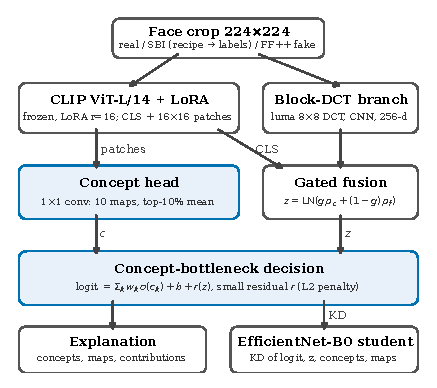
\includegraphics[width=\columnwidth]{fig_architecture.pdf}
\caption{Teacher architecture. The concept head sees only CLIP patch tokens; the DCT feature reaches the logit
through the gated fusion and the residual $r(z)$. The student copies logit, fused feature, concepts and maps.}
\label{fig:arch}
\end{figure}

\subsection{Self-blended images with recipe labels}\label{sec:sbi}
Given a real crop $x\in[0,255]^{224\times224\times3}$ and its landmarks, the engine (\texttt{data/sbi.py}) samples a
region $g$ (full face 0.40, mouth 0.25, eyes and brows 0.20, nose and cheeks 0.15) and fills the convex hull of the
region's landmarks; mouth and eye masks are dilated by 8 and 6 pixels. With probability 0.5 the mask is warped by a
smoothed random displacement field, and it is then blurred with a Gaussian kernel of odd size drawn from 3 to 31 and
scaled to a maximum of 1; the result is the mask $m\in[0,1]^{224\times224}$. A copy $\tilde x$ receives each transform with its own
probability, and at least one transform is forced: a colour shift (0.5; per-channel offset in $[-20,20]$, hue shift
in $[-10^\circ,10^\circ]$, brightness factor in $[-0.10,0.10]$), a texture change (0.5; Gaussian blur with
$\sigma\in[1,2]$ or unsharp masking, equally likely), resampling (0.4; down to a scale in $[0.5,0.9]$ and back) and
an affine shift (0.4; translation up to 3\% and scale in $[0.95,1.05]$). With blend ratio
$a\in\{0.25,0.5,0.75,1\}$,
\begin{equation}
x' = x\odot(1-a\,m) + \tilde x\odot a\,m .
\label{eq:blend}
\end{equation}
Outside the mask, $x'=x$ exactly; this property is used by the restoration test in Section~\ref{sec:restore}.
The recipe defines the concept target $\hat c\in[0,1]^{10}$ in Table~\ref{tab:concepts} and a boundary target
$\hat B = \mathrm{pool}_{16\times16}\bigl(4m(1-m)\bigr)$, normalised to a maximum of 1. Fig.~\ref{fig:sbi} shows five
recipes. Training draws a new recipe for every sample. The student uses a fixed pool of 40,000 self-blends made from
FF++ training reals with a fixed seed, so the teacher's outputs on them can be cached; evaluation uses fixed sets of
2,000 self-blends from FF++ validation reals and 2,000 from FF++ test reals.

\begin{table}[t]
\centering\footnotesize
\caption{Concept targets set from the SBI recipe ($a$: blend ratio).}
\label{tab:concepts}
\begin{tabular}{lll}
\toprule
& Concept & Target \\
\midrule
c1 & blend strength & $a$ \\
c2 & colour mismatch & $a\times$ colour-shift strength $\in[0,1]$ \\
c3 & blur & $a$ if the copy was blurred, else 0 \\
c4 & sharpen & $a$ if sharpened, else 0 \\
c5 & resampling & $a$ if resampled, else 0 \\
c6 & mouth region & 1 if $g$ = mouth, else 0 \\
c7 & eye region & 1 if $g$ = eyes and brows, else 0 \\
c8 & full face & 1 if $g$ = full face, else 0 \\
c9 & geometric misalignment & $a$ if the affine shift was applied, else 0 \\
c10 & irregular boundary & 1 if the mask was warped, else 0 \\
\bottomrule
\end{tabular}
\end{table}

\begin{figure*}[t]
\centering
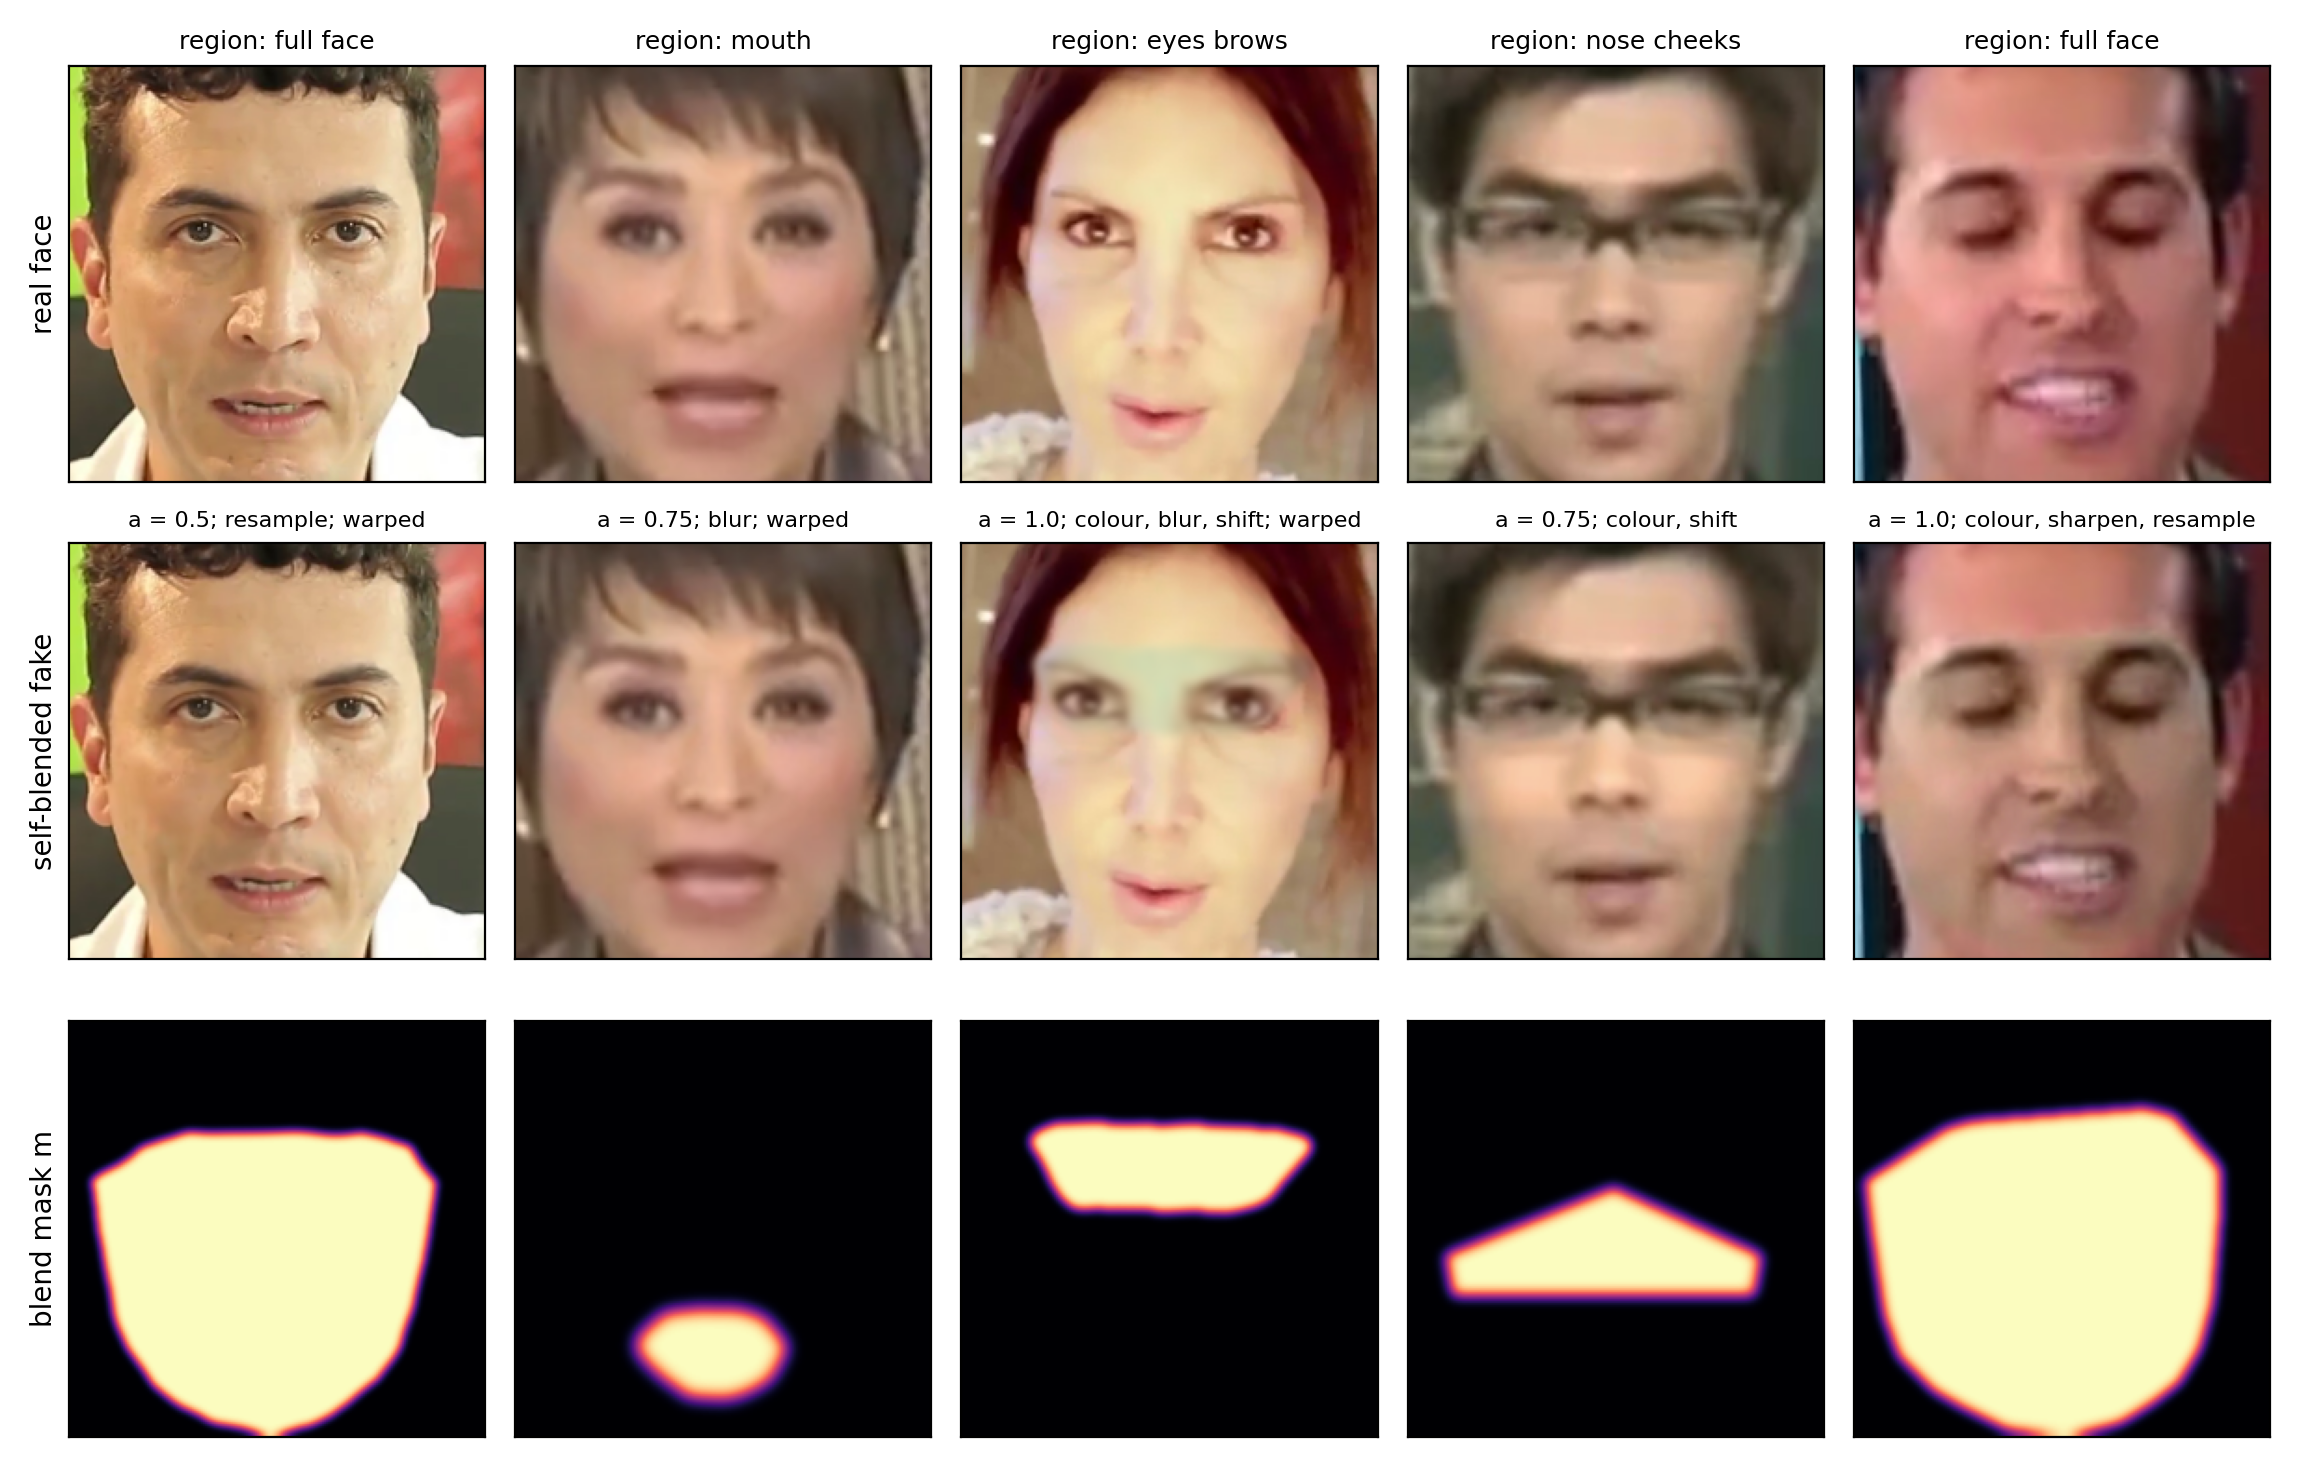
\includegraphics[width=0.82\textwidth]{fig_sbi.png}
\caption{Self-blended training fakes. Top: real FF++ crops. Middle: the self-blend with its recipe ($a$ and the
transforms applied to the copy). Bottom: the blend mask $m$. Each recipe sets the ten concept targets of
Table~\ref{tab:concepts}; nose-and-cheek blends (fourth column) activate no region concept.}
\label{fig:sbi}
\end{figure*}

\subsection{Encoders and fusion}
\textbf{CLIP branch.} The image is normalised and passed through CLIP ViT-L/14 at 224 pixels (timm
\texttt{vit\_large\_patch14\_clip\_224.openai}), whose weights stay frozen. LoRA~\cite{lora} adapters of rank 16
($\alpha=32$, dropout 0.1) on every \texttt{qkv} projection are the only trainable backbone parameters. The branch
returns the CLS feature $h\in\mathbb{R}^{1024}$ and the patch grid $P\in\mathbb{R}^{1024\times16\times16}$.

\textbf{Block-DCT branch.} The luminance $Y = 0.299R+0.587G+0.114B$ (range 0--255) is cut into 8$\times$8 blocks
$X_{ij}$ and transformed with the orthonormal DCT-II matrix $D$ (the 8$\times$8 transform of JPEG; H.264 codes
residuals with integer approximations of the same transform):
\begin{equation}
C_{ij} = D\,X_{ij}\,D^{\top}, \qquad F = \mathrm{BN}\bigl(\log(1+|C|)\bigr)\in\mathbb{R}^{64\times28\times28},
\end{equation}
with the 64 coefficients as channels and a non-affine batch normalisation. Four convolution blocks (1$\times$1 to
64 channels, then three 3$\times$3 stride-2 blocks to 128, 256 and 256 channels, each with BN and GELU) and global
average pooling give $f\in\mathbb{R}^{256}$. The branch runs in float32.

\textbf{Gated fusion.} With $p_c = W_c h$ and $p_f = W_f f$ in $\mathbb{R}^{512}$,
\begin{equation}
g = \sigma\bigl(W_g[p_c;p_f]\bigr), \qquad z = \mathrm{LN}\bigl(g\odot p_c + (1-g)\odot p_f\bigr).
\end{equation}
The gate is computed per dimension and per image. Variants without a frequency branch use $z=\mathrm{LN}(W_c h)$.

\subsection{Concept bottleneck and decision}
A 1$\times$1 convolution maps $P$ to ten concept maps $M\in\mathbb{R}^{10\times16\times16}$ (logits). The score of
concept $k$ is the mean of the largest 10\% of its map (26 of 256 cells), and its activation is
$s_k=\sigma(c_k)$:
\begin{equation}
c_k = \frac{1}{|T_k|}\sum_{u\in T_k} M_{k,u},\qquad T_k = \text{top-}10\%\text{ cells of }M_k .
\end{equation}
The decision is
\begin{equation}
\ell = \sum_{k=1}^{10} w_k\, s_k + b + r(z), \qquad r(z) = W_2\,\mathrm{GELU}(W_1 z),
\label{eq:decision}
\end{equation}
with $W_1\in\mathbb{R}^{64\times512}$. The weights $w_k$ start at 1 and the last layer of $r$ starts at zero, so
training begins from a concept-only decision. We measure how much of the logit passes through the concepts with the
concept share
\begin{equation}
\rho = \mathrm{Var}\Bigl(\sum_k w_k s_k\Bigr)\Big/\mathrm{Var}(\ell),
\end{equation}
computed over the frames of a test set.

\subsection{Training objective and optimisation}\label{sec:objective}
A cell-balanced sampler fills each batch of 32 from five cells, real, SBI, Deepfakes, Face2Face and FaceSwap, with
weights 3:2:1:1:1; small cells are cycled. Concept and boundary targets exist only for SBI samples, and masked
binary cross-entropy $\mathcal{B}_{\mathrm{SBI}}$ averages over those samples. The loss is
\begin{align}
\mathcal{L} = {} & \mathcal{B}(\ell, y) + \lambda_c\,\mathcal{B}_{\mathrm{SBI}}(c,\hat c)
+ \lambda_m\,\mathcal{B}_{\mathrm{SBI}}(M_{\mathrm{b}},\hat B) \nonumber\\
& + \lambda_w \|w\|_1 + \lambda_r\, \mathbb{E}\bigl[r(z)^2\bigr],
\label{eq:loss}
\end{align}
where $M_{\mathrm{b}}$ is the first concept map compared with the boundary target, $\lambda_c=\lambda_m=0.5$ and
$\lambda_w=10^{-4}$. The residual weight $\lambda_r$ was $10^{-3}$ in the first concept models (G1, G2) and
$10^{-2}$ from then on: on FF++ validation, a G1 run with $\lambda_r=10^{-2}$ matched the video AUC of
$\lambda_r=10^{-3}$ (both 1.000 to three decimals) and raised the validation concept share from 0.248 to 0.639.

AdamW~\cite{adamw} uses weight decay 0.05 and learning rates $2\times10^{-4}$ (LoRA), $2\times10^{-3}$ (DCT branch)
and $10^{-3}$ (fusion and heads), with one epoch of linear warm-up followed by cosine decay to 1\% of each rate. A
run has 12 epochs of 1,500 steps in bf16 with gradient clipping at 1.0. An exponential moving average of the
weights (decay 0.999) is evaluated on FF++ validation after every epoch and the best epoch is kept. Augmentation:
horizontal flip (0.5), colour jitter (0.1), Gaussian blur (0.1) and JPEG re-encoding (0.3, quality 60--100). One run
takes 1.9--2.0\,h on one NVIDIA RTX 4500 Ada (24\,GB).

\subsection{Model selection}\label{sec:select}
For the fine-tuned CLIP models, clean FF++ validation video AUC reaches 0.999--1.000 within a few epochs (C1: 1.000
from the third epoch), so it does not separate epochs or candidates. The final teacher F1 is therefore selected on
\begin{equation}
S = \tfrac{1}{3}\bigl(\mathrm{AUC}_{\mathrm{val}} + \mathrm{AUC}_{\mathrm{val}}^{\mathrm{H.264\,40}} +
\mathrm{AUC}_{\mathrm{SBI\text{-}val}}\bigr),
\end{equation}
the mean of clean validation AUC, validation AUC after H.264 CRF-40 encoding, and AUC of 2,000 validation
self-blends against the validation reals. Its seed-42 run reaches $S=0.961$ at epoch 8 (0.999, 0.906 and 0.979).
Because $S$ contains an H.264 term, F1 is not blind to H.264 as a degradation type, although no test video is
seen.

\subsection{Single-frame H.264 augmentation}
F1h adds one augmentation to F1: with probability 0.3 a training crop is encoded as a single H.264 frame with
libx264 (through PyAV, preset veryfast) at a CRF drawn uniformly from 24 to 38 and decoded back. A single frame is
intra-coded, so this approximates but does not reproduce the video-level test encoding, which also has inter-frame
prediction. CRF 40 never occurs in training.

\subsection{Distillation into a CPU student}\label{sec:kd}
The student is an EfficientNet-B0~\cite{efficientnet} (ImageNet weights) whose 1280$\times$7$\times$7 feature map
feeds the same concept head (top 10\% = 5 of 49 cells) and decision layer, with
$z_S=\mathrm{LN}(W\,\mathrm{GAP}(\cdot))\in\mathbb{R}^{512}$. It trains on 86,058 crops (FF++ training crops plus
the 40,000-image SBI pool) for 15 epochs of 1,500 steps, batch 64, learning rate $10^{-3}$. Each input is degraded:
unchanged (0.20), JPEG quality 20--60 (0.35), downscaled to 25--50\% (0.25), or downscaled to 50\% and then JPEG
30--50 (0.20). The teacher's outputs on the clean crop are read from a cache built once with the EMA weights. With
$T=4$ and $\mathrm{KL}_T$ the Bernoulli KL divergence between $\sigma(\ell_T/T)$ and $\sigma(\ell_S/T)$,
\begin{align}
\mathcal{L}_S = {} & 0.5\,\mathcal{B}(\ell_S,y) + 0.5\,T^2\,\mathrm{KL}_T + \|z_S - z_T\|^2 \nonumber\\
& + 0.5\,\mathcal{B}\bigl(c_S, \sigma(c_T)\bigr) + 0.5\,\bigl\|\sigma(M_S) - \mathrm{pool}(\sigma(M_T))\bigr\|^2 .
\label{eq:kd}
\end{align}
S0 drops the teacher and trains on recipe labels ($\mathcal{B}$ weight 1, concept and map weights 0.5); S2 keeps only
the logit term. S3h replaces a quarter of the degraded inputs with single-frame H.264 at CRF 24--38. The student is
exported to ONNX for the application.

\subsection{Models compared}\label{sec:models}
Table~\ref{tab:models} defines every model. Within the CLIP family each model changes one component of its parent.
B2, B2f, G3, F2 and D2 test domain alignment: a gradient-reversal domain classifier~\cite{ganin} (weight 0.1) plus
MMD~\cite{mmd} (weight 0.1) between manipulation domains, applied to different features. D2 uses weight 0.01 and
two domains (FF++ and a pool of unlabelled Celeb-DF crops that excludes every test video).

\begin{table}[t]
\centering\footnotesize
\setlength{\tabcolsep}{3pt}
\caption{Models. All use the same splits, crops, sampler and evaluation code. Seeds: 3 unless marked $^1$.}
\label{tab:models}
\begin{tabular}{ll}
\toprule
ID & Definition \\
\midrule
B1 & Swin-B~\cite{swin}, real + FF++ fakes, lr $10^{-4}$, 10 epochs \\
B2 / B2f$^1$ & B1 + DANN/MMD on all 4 domains / on fake domains \\
R1 & frozen CLIP ViT-L/14 + linear head (UnivFD-style~\cite{univfd}) \\
R2 & EfficientNet-B4, real + SBI only, 1:1 (SBI-style~\cite{sbi}) \\
C1 & CLIP ViT-L/14 + LoRA, linear head, real + FF++ fakes \\
C2 & C1 + SBI cell \\
G1 & C2 + concept head and decision, $\lambda_r=10^{-3}$ \\
G2 & G1 + block-DCT branch + gated fusion \\
G2-fft$^1$ & G1 + FFT-magnitude branch + gated fusion, $\lambda_r=10^{-2}$ \\
G3 & G2-fft + DANN/MMD on $z$ over fake domains \\
A3 & G3 with a linear head on $z$ and no concept loss \\
F1 & G2 + $\lambda_r=10^{-2}$ + selection score $S$ (final teacher) \\
F1h & F1 + single-frame H.264 augmentation \\
F2$^1$ & F1 + DANN/MMD on mean-pooled patch tokens \\
D2 & F1 + unlabelled Celeb-DF crops, DANN/MMD 0.01 \\
X1 & F1 recipe trained on FF++ + all DFD videos (DFD not a test set) \\
S0--S3xx & EfficientNet-B0 students (Section~\ref{sec:kd}, Table~\ref{tab:students}) \\
\bottomrule
\end{tabular}
\end{table}

% =====================================================================================================
\section{Results}\label{sec:results}

\begin{table*}[t]
\centering
\footnotesize
\caption{Video AUC under the leak-free protocol (mean$\pm$sample std over 3 seeds). Cross is the mean of the DFD and Celeb-DF AUCs; its 95\% CI comes from 1,000 stratified bootstrap resamples of the test videos applied to the seed-mean AUC. All models share the FF++ training videos, face crops, sampler and selection code; R2 trains on real faces and their self-blends only.}
\label{tab:main}
\begin{tabular}{llccccc}
\toprule
ID & Model & FF++ test & DFD & Celeb-DF & Cross & Cross 95\% CI \\
\midrule
B1 & Swin-B, FF++ fakes & 0.997$\pm$0.003 & 0.903$\pm$0.020 & 0.805$\pm$0.016 & 0.854$\pm$0.012 & [0.837, 0.872] \\
R1 & frozen CLIP, linear probe & 0.944$\pm$0.000 & 0.857$\pm$0.001 & 0.743$\pm$0.002 & 0.800$\pm$0.001 & [0.775, 0.825] \\
R2 & SBI reprod., EffNet-B4 & 0.906$\pm$0.008 & 0.810$\pm$0.009 & 0.616$\pm$0.015 & 0.713$\pm$0.009 & [0.684, 0.742] \\
\midrule
C1 & CLIP ViT-L/14 + LoRA & 1.000$\pm$0.000 & 0.931$\pm$0.010 & 0.880$\pm$0.011 & 0.906$\pm$0.009 & [0.892, 0.920] \\
F1 & final teacher & 0.997$\pm$0.004 & 0.951$\pm$0.004 & 0.878$\pm$0.017 & 0.914$\pm$0.010 & [0.898, 0.930] \\
F1h & F1 + H.264 augmentation & 0.993$\pm$0.007 & 0.939$\pm$0.006 & 0.886$\pm$0.005 & 0.912$\pm$0.004 & [0.896, 0.928] \\
\bottomrule
\end{tabular}
\end{table*}


\subsection{Comparison with baselines}
Table~\ref{tab:main} reports the main comparison. Every model scores 0.906 or higher on FF++ test, and the
fine-tuned models B1, C1, F1 and F1h score 0.993 or higher, so the cross-dataset columns decide the ranking. F1 reaches 0.914 cross AUC, 0.060 above
Swin-B (paired 95\% CI [+0.042, +0.079]), 0.114 above the frozen-CLIP probe R1 and 0.201 above R2. R2 reproduces the
SBI training recipe with our engine, our 46,058 FF++ training crops and a 10-epoch budget; its Celeb-DF AUC of 0.616
is far below the value reported by Shiohara and Yamasaki~\cite{sbi}, who trained on the full FF++ release with their
own pipeline, and we report it as a reference point under our data, not as a measurement of their method. R1 varies
by less than 0.002 between seeds because only its linear head is trained.

Against C1, which shares the backbone and differs in everything this paper adds, F1 gains 0.019 on DFD and loses
0.002 on Celeb-DF; the cross difference of +0.009 has CI [$-$0.007, +0.024] and $p=0.308$. On clean video, the
backbone change from Swin-B to CLIP with LoRA (+0.052 cross, CI [+0.037, +0.067]) accounts for the measurable gain.
The remaining sections test what the additions change other than clean AUC.

\begin{table*}[t]
\centering
\footnotesize
\caption{Paired change in seed-mean video AUC, later model minus earlier (3 seeds each, the same resampled videos for both models). $^{*}$: the 95\% paired bootstrap CI excludes zero. CI and two-sided bootstrap $p$ refer to the cross column. Concept share: variance of the concept part of the logit divided by the variance of the logit on FF++ test frames, for the later model (-- for linear heads).}
\label{tab:ablation}
\begin{tabular}{llcccccc}
\toprule
Pair & Change & DFD & Celeb-DF & Cross & Cross 95\% CI & $p$ & Concept share \\
\midrule
C2 vs.\ C1 & + SBI pseudo-fakes in the batch & +0.028$^{*}$ & $-$0.023 & +0.003 & [$-$0.014, +0.019] & 0.752 & -- \\
G1 vs.\ C2 & + concept bottleneck (residual 1e-3) & $-$0.004$^{*}$ & +0.022$^{*}$ & +0.009$^{*}$ & [+0.004, +0.014] & 0.000 & 0.36$\pm$0.15 \\
G2 vs.\ G1 & + block-DCT branch, gated fusion & +0.010$^{*}$ & +0.002 & +0.006$^{*}$ & [+0.002, +0.010] & 0.000 & 0.36$\pm$0.13 \\
F1 vs.\ G2 & residual 1e-3 $\to$ 1e-2, harder selection & $-$0.015$^{*}$ & $-$0.003 & $-$0.009$^{*}$ & [$-$0.017, $-$0.001] & 0.022 & 0.84$\pm$0.00 \\
G3 vs.\ A3 & concept head vs.\ linear head (both + DANN) & +0.013$^{*}$ & +0.019$^{*}$ & +0.016$^{*}$ & [+0.006, +0.025] & 0.000 & 1.00$\pm$0.00 \\
\midrule
C1 vs.\ B1 & Swin-B $\to$ CLIP ViT-L/14 + LoRA & +0.028$^{*}$ & +0.075$^{*}$ & +0.052$^{*}$ & [+0.037, +0.067] & 0.000 & -- \\
F1 vs.\ C1 & all additions together & +0.019$^{*}$ & $-$0.002 & +0.009 & [$-$0.007, +0.024] & 0.308 & 0.84$\pm$0.00 \\
F1h vs.\ F1 & + single-frame H.264 augmentation & $-$0.011$^{*}$ & +0.008 & $-$0.002 & [$-$0.008, +0.004] & 0.588 & 0.81$\pm$0.00 \\
\bottomrule
\end{tabular}
\end{table*}


\subsection{Ablation}
Table~\ref{tab:ablation} compares each model with its parent. Adding the SBI cell to C1 moves DFD and Celeb-DF in
opposite directions (+0.028 and $-$0.023); cross AUC does not change (+0.003). The concept bottleneck (G1 vs.\ C2) adds
+0.009 cross with a Celeb-DF gain of +0.022, and the DCT branch (G2 vs.\ G1) adds +0.006, both statistically
significant. In G1 and G2, however, the concept part explains only 0.36 of the logit variance on FF++ test: with
$\lambda_r=10^{-3}$ the residual carries most of the decision.

F1 raises $\lambda_r$ to $10^{-2}$ and uses the selection score $S$. Its concept share rises to 0.84 with a seed
spread below 0.01, and its cross AUC falls by 0.009 against G2 (CI [$-$0.017, $-$0.001]). F1 was fixed on FF++
validation before any test score was computed; we keep it as the final teacher and report the cost. The cleanest
test of the bottleneck is G3 against A3, two models that differ only in the head: replacing the linear head on $z$
with the concept head and its recipe supervision adds +0.016 cross (CI [+0.006, +0.025]), with gains on both test
sets. In all three G3 runs the residual contributes no variance to the logit ($\rho=1.00$) and the fusion gate closes
on the CLIP feature; the domain loss is met by emptying the residual path, and the decision runs entirely through the
concepts. A3 has no concept path, and the same domain loss acts on its only path to the logit.

\begin{table*}[t]
\centering
\footnotesize
\caption{Domain alignment and training data. $\Delta$ is the change in mean cross AUC against the parent model (B1 for B2 and B2f, G2-fft for G3, F1 for F2 and D2); for X1, DFD is training data, so the change is reported on Celeb-DF against F1. The D2 pool of unlabelled Celeb-DF crops excludes every test video.}
\label{tab:align}
\begin{tabular}{lllcccc}
\toprule
ID & Change & Seeds & DFD & Celeb-DF & Cross & $\Delta$ \\
\midrule
B2 & B1 + DANN/MMD, real is a domain & 1 & 0.870 & 0.787 & 0.828 & $-$0.025 \\
B2f & B1 + DANN/MMD on fake domains only & 1 & 0.904 & 0.826 & 0.865 & +0.011 \\
G3 & G2-fft + DANN/MMD on $z$, fake domains & 3 & 0.963$\pm$0.012 & 0.860$\pm$0.005 & 0.912$\pm$0.006 & $-$0.003 \\
F2 & F1 + DANN/MMD on patch tokens & 1 & 0.813 & 0.654 & 0.733 & $-$0.181 \\
D2 & F1 + unlabelled Celeb-DF crops, DANN/MMD & 3 & 0.955$\pm$0.003 & 0.832$\pm$0.024 & 0.893$\pm$0.013 & $-$0.021 \\
\midrule
X1 & F1 recipe trained on FF++ + all of DFD & 3 & (train) & 0.944$\pm$0.005 & -- & +0.066 (CDF) \\
\bottomrule
\end{tabular}
\end{table*}


\subsection{Domain alignment and training data}\label{sec:data_vs_arch}
Table~\ref{tab:align} collects every domain-alignment variant. Treating real faces as one of the domains (B2) costs
0.025 cross AUC: the reversed gradient pushes the features to hide the real/fake distinction that the classifier
needs. Restricting the domain loss to fake domains (B2f, one seed) adds +0.011, inside the seed spread of B1
(0.012). On the CLIP models, alignment on $z$ (G3) changes cross AUC by $-$0.003 against its FFT parent, alignment
on the patch tokens that feed the concept head (F2) costs 0.181, and unsupervised alignment to Celeb-DF (D2) lowers
Celeb-DF AUC from 0.878 to 0.832 although its target pool comes from Celeb-DF itself.

Training data has a larger effect than any architectural change in this study. X1 trains the F1 recipe on FF++ plus
all DFD videos and reaches 0.944 on Celeb-DF over three seeds, 0.066 above F1. The leaked
checkpoint of Section~\ref{sec:leak}, which also trained on FF++ and DFD, scores 0.956 on Celeb-DF. Both results
point to the size and variety of our FF++ subset (Table~\ref{tab:data}) as the main limit on cross-dataset AUC.

\begin{table}[t]
\centering
\footnotesize
\setlength{\tabcolsep}{3pt}
\caption{Cross-dataset video AUC with degraded test frames (mean$\pm$sample std, 3 seeds). Down 0.25: downscale to 25\% and back. F1h trains with CRF 24--38, never 40.}
\label{tab:robust}
\begin{tabular}{lcccc}
\toprule
Model & Clean & JPEG 30 & Down 0.25 & H.264 40 \\
\midrule
B1 & 0.854$\pm$0.012 & 0.776$\pm$0.033 & 0.757$\pm$0.030 & 0.561$\pm$0.012 \\
R1 & 0.800$\pm$0.001 & 0.757$\pm$0.001 & 0.741$\pm$0.000 & 0.681$\pm$0.001 \\
R2 & 0.713$\pm$0.009 & 0.710$\pm$0.011 & 0.719$\pm$0.010 & 0.555$\pm$0.014 \\
\midrule
C1 & 0.906$\pm$0.009 & 0.789$\pm$0.026 & 0.823$\pm$0.012 & 0.624$\pm$0.014 \\
C2 & 0.908$\pm$0.003 & 0.898$\pm$0.017 & 0.886$\pm$0.007 & 0.661$\pm$0.018 \\
G1 & 0.917$\pm$0.004 & 0.901$\pm$0.005 & 0.895$\pm$0.013 & 0.652$\pm$0.011 \\
G2 & 0.923$\pm$0.009 & 0.909$\pm$0.008 & 0.895$\pm$0.014 & 0.653$\pm$0.026 \\
F1 & 0.914$\pm$0.010 & 0.901$\pm$0.008 & 0.878$\pm$0.010 & 0.644$\pm$0.020 \\
F1h & 0.912$\pm$0.004 & 0.894$\pm$0.003 & 0.875$\pm$0.009 & 0.688$\pm$0.006 \\
\bottomrule
\end{tabular}
\end{table}


\begin{figure}[t]
\centering
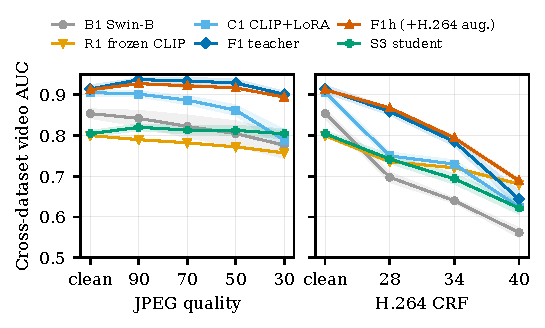
\includegraphics[width=\columnwidth]{fig_robustness.pdf}
\caption{Cross-dataset video AUC as test compression increases. Bands: $\pm$1 std over 3 seeds.}
\label{fig:robust}
\end{figure}

\subsection{Robustness to compression and resizing}
Table~\ref{tab:robust} and Fig.~\ref{fig:robust} report cross AUC on degraded test frames. At JPEG quality 30,
C1 falls from 0.906 to 0.789 while F1 keeps 0.901. All CLIP models train with the same JPEG augmentation at quality
60--100, and the chain C1, C2, G1, G2, F1 locates the gain: adding self-blends (C2) raises JPEG-30 AUC to 0.898
(paired +0.109 against C1, CI [+0.089, +0.130]), and the concept head and DCT branch move it by at most 0.011 more
(G2: 0.909). After downscaling to 25\%, C2, G1 and G2 reach 0.886--0.895 and F1 0.878, against 0.823 for C1. The
cues learned from self-blends therefore survive re-encoding and resizing better than the cues learned from FF++
fakes alone, and the frequency branch, which reads the same DCT coefficients that JPEG quantises, adds no measurable
JPEG robustness on top of them.

H.264 at CRF 40 is the hardest condition for every model. F1 reaches 0.644, C1 0.624 and C2 0.661. Single-frame H.264
training (F1h) raises F1 to 0.688 (paired +0.045, CI [+0.025, +0.063]) and reduces the seed spread from 0.020 to
0.006, with a clean cross change of $-$0.002 (CI [$-$0.008, +0.004]). The frozen probe R1 reaches 0.681 at CRF 40,
higher than every fine-tuned model except F1h, while it is the second weakest model on clean video: fine-tuning
raises clean AUC and makes the features more sensitive to strong inter-frame compression.

\begin{table}[t]
\centering
\footnotesize
\setlength{\tabcolsep}{3pt}
\caption{Expected calibration error of the video score (15 equal-width bins, seed 42; lower is better), raw / after the temperature $T$ fitted on FF++ validation frames.}
\label{tab:ece}
\begin{tabular}{lcccc}
\toprule
Model & $T$ & FF++ & DFD & Celeb-DF \\
\midrule
B1 & 4.75 & 0.057 / 0.089 & 0.237 / 0.233 & 0.578 / 0.489 \\
R1 & 1.00 & 0.093 / 0.093 & 0.182 / 0.182 & 0.394 / 0.394 \\
R2 & 1.00 & 0.151 / 0.151 & 0.067 / 0.067 & 0.088 / 0.088 \\
C1 & 1.00 & 0.037 / 0.037 & 0.261 / 0.261 & 0.527 / 0.527 \\
C2 & 1.00 & 0.082 / 0.082 & 0.075 / 0.075 & 0.069 / 0.069 \\
G1 & 1.00 & 0.108 / 0.108 & 0.158 / 0.158 & 0.230 / 0.230 \\
G2 & 1.00 & 0.107 / 0.107 & 0.157 / 0.157 & 0.216 / 0.216 \\
F1 & 1.04 & 0.068 / 0.071 & 0.075 / 0.074 & 0.161 / 0.159 \\
F1h & 1.00 & 0.075 / 0.075 & 0.048 / 0.048 & 0.059 / 0.059 \\
S3 & 1.66 & 0.074 / 0.121 & 0.074 / 0.071 & 0.105 / 0.075 \\
\bottomrule
\end{tabular}
\end{table}


\subsection{Calibration}
Table~\ref{tab:ece} reports the expected calibration error~\cite{guo}
$\mathrm{ECE}=\sum_{b=1}^{15}\frac{|B_b|}{n}\,\bigl|\bar y_b - \bar p_b\bigr|$ of the video score, where $B_b$ are
the videos whose score falls into bin $b$. On FF++ test all models stay below 0.16. On Celeb-DF, the models trained
without self-blends are badly calibrated (B1 0.578, C1 0.527, R1 0.394). Adding self-blends to C1 lowers the error
to 0.069 (C2). The concept models are worse than C2 (G1 0.230, G2 0.216, F1 0.161) and F1h is better (0.059). We
have not isolated the cause of the gap between C2 and the concept models; their logit is a sum of up to ten positive
terms and a bias rather than one linear output, which changes how the score scales on unseen data. In this study,
good calibration on Celeb-DF comes from the self-blended training data and from H.264 training, not from the concept
bottleneck. All ECE values are from seed 42.

Temperature scaling fitted on FF++ validation does not repair the cross-dataset error (B1: 0.578 to 0.489) because
FF++ validation is almost perfectly separated, so the fitted temperature carries little information about unseen
data. ECE measures whether the score can be read as a frequency, not ranking: R2 has an ECE of 0.088 on Celeb-DF and
an AUC of 0.616.

\begin{table*}[t]
\centering
\footnotesize
\caption{EfficientNet-B0 students (4.71\,M parameters, 0.39\,GFLOPs; 3 seeds each). Teacher F1: 306.94\,M parameters, 81.46\,GFLOPs. H.264 40 is the cross AUC at CRF 40 (-- where not evaluated). S0x and S3xx train on DFD, so DFD is not a test set for them.}
\label{tab:students}
\begin{tabular}{llcccc}
\toprule
ID & Training signal & FF++ test & DFD & Celeb-DF & Cross, H.264 40 \\
\midrule
S0 & no teacher & 0.984$\pm$0.004 & 0.867$\pm$0.027 & 0.751$\pm$0.027 & 0.606$\pm$0.015 \\
S2 & KD: logit only & 0.984$\pm$0.007 & 0.859$\pm$0.010 & 0.752$\pm$0.012 & 0.613$\pm$0.010 \\
S3 & KD: logit, $z$, concepts, maps & 0.978$\pm$0.007 & 0.844$\pm$0.013 & 0.765$\pm$0.025 & 0.622$\pm$0.015 \\
\midrule
S3h & S3 + H.264 inputs & 0.984$\pm$0.007 & 0.888$\pm$0.024 & 0.769$\pm$0.015 & 0.610$\pm$0.023 \\
S3hh & S3h, teacher F1h & 0.980$\pm$0.008 & 0.883$\pm$0.030 & 0.775$\pm$0.022 & 0.619$\pm$0.008 \\
\midrule
S3x & S3, teacher X1 & 0.987$\pm$0.003 & 0.864$\pm$0.013 & 0.752$\pm$0.027 & -- \\
S0x & S0 + DFD in training & 0.990$\pm$0.003 & (train) & 0.805$\pm$0.028 & -- \\
S3xx & S3x + DFD in training & 0.992$\pm$0.003 & (train) & 0.797$\pm$0.029 & -- \\
\bottomrule
\end{tabular}
\end{table*}


\subsection{Distillation and efficiency}
Table~\ref{tab:students} lists the students. The EfficientNet-B0 student has 4.71\,M parameters and 0.39\,GFLOPs per
crop against 306.94\,M and 81.46\,GFLOPs for F1, a factor of 65 in parameters. On one RTX 4500 Ada it processes
3,939 crops per second against 286 for F1, and its ONNX export takes 4.2\,ms per crop on a CPU with four threads
at batch size 1.

No student comes close to the teacher: S3 reaches 0.804 cross AUC against 0.914. Full distillation (S3) does not
beat the teacher-free S0 on clean data (cross $-$0.005, CI [$-$0.014, +0.005]); S3 is ahead on Celeb-DF by 0.014
and behind on DFD. Its effect is on consistency and concept behaviour: the seed spread of cross AUC falls from 0.026
to 0.008, and on 2,000 FF++ test crops the Spearman correlation between the student's and the teacher's ten concept
scores rises from 0.645 (S0) to 0.790 (S3). The overlap of the top concept maps does not rise (IoU 0.140 for S0,
0.113 for S3).

Three further variants test where the student's limits come from. H.264 inputs (S3h) improve clean DFD AUC by
0.045 but not CRF-40 AUC (0.610 vs.\ 0.622). Distilling S3h from the H.264-trained teacher F1h (S3hh) changes CRF-40
AUC by +0.009 (CI [$-$0.003, +0.019]). Distilling from the stronger X1 teacher (S3x) leaves Celeb-DF at 0.752, while
adding DFD to the student's own training data (S0x) raises it to 0.805. In all three cases the student follows its
training data, not its teacher's accuracy.

% =====================================================================================================
\section{Interventional Analysis of the Decision}\label{sec:interv}

The analyses above treat each model as a scorer. This section asks how F1 reaches its scores: which internal
variables the logit depends on, and whether the image regions named by the concept maps contain the evidence.

\subsection{Estimands and assumptions}
Equation~\eqref{eq:decision} is linear in the activations $s_k$, so an intervention that sets one activation to
zero, $\mathrm{do}(s_k=0)$, has the exact effect
\begin{equation}
\ell^{\mathrm{do}(s_k=0)} = \ell - w_k s_k
\label{eq:do}
\end{equation}
on every frame, with all other activations and $r(z)$ held fixed. We define two further interventions: concepts only,
$\mathrm{do}(r=0)$, with logit $\sum_k w_k s_k + b$; and residual only, $\mathrm{do}(s=0)$, with logit $b+r(z)$. Each
intervened logit is turned into a video score as before. We report three estimands per intervention: the change in
video AUC; the mean logit contribution $w_k s_k$ on fake frames minus that on real frames, $\Delta\ell_k$; and the
flip rate, the share of fake videos above the FF++-validation threshold that fall below it after the intervention.

These quantities are computed from the stored $s_k$, logits and concept parts of every test frame, with $w$ and $b$
read from each checkpoint; the stored concept parts are reproduced to within $10^{-6}$. The interventions act on
the model's internal variables. They identify how the trained decision depends on each concept unit; they do not
identify which property of the input image caused that unit to fire. The image-level question is addressed by the
restoration test in Section~\ref{sec:restore}, where the counterfactual image is known.

\begin{table*}[t]
\centering
\footnotesize
\setlength{\tabcolsep}{4pt}
\caption{Decision decomposition by intervention on the bottleneck (video AUC, mean$\pm$sample std over 3 seeds). Concepts only: $r(z)$ set to 0; residual only: all $s_k$ set to 0. Concept share on Celeb-DF frames.}
\label{tab:decomp}
\begin{tabular}{llccccccc}
\toprule
Model & Test frames & \multicolumn{3}{c}{DFD: full / concepts / residual} & \multicolumn{3}{c}{Celeb-DF: full / concepts / residual} & Share \\
\midrule
F1 & clean & 0.951$\pm$0.004 & 0.950$\pm$0.004 & 0.943$\pm$0.006 & 0.878$\pm$0.017 & 0.880$\pm$0.016 & 0.846$\pm$0.016 & 0.77$\pm$0.02 \\
F1 & H.264 40 & 0.646$\pm$0.012 & 0.646$\pm$0.013 & 0.639$\pm$0.005 & 0.641$\pm$0.029 & 0.640$\pm$0.026 & 0.649$\pm$0.032 & 0.71$\pm$0.03 \\
F1h & clean & 0.939$\pm$0.006 & 0.940$\pm$0.006 & 0.902$\pm$0.031 & 0.886$\pm$0.005 & 0.887$\pm$0.006 & 0.865$\pm$0.006 & 0.75$\pm$0.00 \\
F1h & H.264 40 & 0.692$\pm$0.006 & 0.692$\pm$0.006 & 0.667$\pm$0.007 & 0.685$\pm$0.007 & 0.684$\pm$0.009 & 0.679$\pm$0.018 & 0.88$\pm$0.02 \\
\bottomrule
\end{tabular}
\end{table*}


\subsection{Concepts against residual}
Table~\ref{tab:decomp} decomposes the decision. With the residual removed, the ten concepts alone reproduce F1's
clean AUC on both test sets (DFD 0.950 vs.\ 0.951; Celeb-DF 0.880 vs.\ 0.878). With all concepts removed, the
residual alone loses 0.008 on DFD and 0.032 on Celeb-DF. The concept share on Celeb-DF frames is 0.77. The ranking
of test videos therefore depends on the named concepts, and the DCT feature, which reaches the logit only through
$r(z)$, contributes no measurable ranking information on clean frames.

Under H.264 CRF 40 the picture changes. For F1, concepts only, residual only and the full model all fall to
0.640--0.649 on Celeb-DF; both paths fail together. F1h keeps the concept path working (0.684 concepts only vs.\
0.685 full on Celeb-DF; 0.692 vs.\ 0.692 on DFD), and its concept share on compressed Celeb-DF frames rises to 0.88.
The gain of H.264 training is therefore a gain of the concept path. The residual-only variant flips every flagged
fake video to real (flip rate 1.000 in all conditions), because $b=-1.89$ for the seed-42 run and $r(z)$ alone does
not reach the threshold; its AUC, not its flip rate, is the informative quantity.

\begin{table*}[t]
\centering
\footnotesize
\setlength{\tabcolsep}{4pt}
\caption{Effect of switching off one concept, do$(s_k{=}0)$, in F1 (mean over 3 seeds, clean test frames). $\bar w_k$: learned weight. $\Delta\ell$: mean logit contribution $w_k s_k$ on fake frames minus on real frames. Flip: share of fake videos flagged by the full model (FF++-val threshold) that fall below the threshold after the intervention. $\Delta$AUC: change in Celeb-DF video AUC.}
\label{tab:effects}
\begin{tabular}{llccccccc}
\toprule
& Concept & $\bar w_k$ & DFD $\Delta\ell$ & DFD flip (\%) & CDF $\Delta\ell$ & CDF flip (\%) & CDF $\Delta$AUC \\
\midrule
c1 & blend strength & 2.29 & 0.89 & 2.8 & 0.46 & 10.2 & +0.003 \\
c2 & colour mismatch & 2.37 & 0.72 & 1.0 & 0.16 & 0.8 & $-$0.000 \\
c3 & blur & 1.98 & 0.23 & 0.3 & 0.05 & 0.6 & +0.001 \\
c4 & sharpen & 1.68 & 0.23 & 0.8 & 0.07 & 1.5 & +0.001 \\
c5 & resampling & 2.05 & 0.45 & 1.0 & 0.12 & 1.4 & +0.003 \\
c6 & mouth region & 0.99 & 0.03 & 0.9 & $-$0.01 & 1.4 & +0.002 \\
c7 & eye region & 1.39 & 0.03 & 0.7 & 0.01 & 1.8 & +0.002 \\
c8 & full face & 2.06 & 1.17 & 2.7 & 0.73 & 13.1 & $-$0.014 \\
c9 & geometric misalign. & 2.27 & 0.70 & 1.3 & 0.26 & 3.5 & $-$0.000 \\
c10 & irregular boundary & 2.00 & 0.79 & 3.0 & 0.38 & 9.0 & +0.002 \\
\bottomrule
\end{tabular}
\end{table*}


\subsection{Effect of single concepts}
Table~\ref{tab:effects} switches off one concept at a time. All ten learned weights are positive (0.99 to 2.37), so
every active concept pushes towards ``fake''. On DFD, the largest fake-minus-real contributions come from full face
(1.17), blend strength (0.89), irregular boundary (0.79) and colour mismatch (0.72). On Celeb-DF the same concepts
lead, at about half the magnitude, which matches the visual quality gap between the two datasets.

Removing any single concept changes Celeb-DF AUC by at most 0.014: the concepts are redundant for ranking. They are
not redundant for decisions at the operating point. Switching off full face flips 13.1\% of the Celeb-DF fakes that
F1 flags, blend strength 10.2\% and irregular boundary 9.0\%; the colour, blur, sharpening, resampling and region
concepts each flip less than 2\%. Only the full-face removal lowers Celeb-DF AUC ($-$0.014); the others leave it
within $\pm$0.003. Celeb-DF fakes are full-face swaps, and the concept whose recipe meaning matches that manipulation
carries most of the decision.

\begin{table*}[t]
\centering
\footnotesize
\setlength{\tabcolsep}{4pt}
\caption{Mean concept score $s_k$ of F1 (seed 42) per test group, frame level. The concepts were trained only on self-blended images; FF++ fakes and all DFD/Celeb-DF videos carry no concept labels.}
\label{tab:bymethod}
\begin{tabular}{lccccccccccc}
\toprule
Group & Frames & c1 & c2 & c3 & c4 & c5 & c6 & c7 & c8 & c9 & c10 \\
\midrule
FF++ real & 4,400 & 0.03 & 0.01 & 0.00 & 0.01 & 0.01 & 0.02 & 0.01 & 0.02 & 0.01 & 0.03 \\
FF++ Deepfakes & 3,591 & 0.67 & 0.58 & 0.21 & 0.38 & 0.44 & 0.05 & 0.14 & 0.91 & 0.68 & 0.71 \\
FF++ Face2Face & 640 & 0.49 & 0.47 & 0.11 & 0.55 & 0.32 & 0.20 & 0.45 & 0.75 & 0.65 & 0.63 \\
FF++ FaceSwap & 192 & 0.36 & 0.47 & 0.06 & 0.46 & 0.18 & 0.16 & 0.41 & 0.60 & 0.50 & 0.52 \\
\midrule
DFD real & 11,007 & 0.11 & 0.02 & 0.01 & 0.03 & 0.03 & 0.05 & 0.04 & 0.10 & 0.04 & 0.12 \\
DFD fake & 29,023 & 0.49 & 0.29 & 0.10 & 0.16 & 0.22 & 0.06 & 0.06 & 0.66 & 0.34 & 0.50 \\
\midrule
Celeb-real & 3,412 & 0.12 & 0.01 & 0.01 & 0.05 & 0.04 & 0.06 & 0.04 & 0.08 & 0.04 & 0.12 \\
YouTube-real & 2,184 & 0.17 & 0.02 & 0.02 & 0.06 & 0.05 & 0.06 & 0.05 & 0.13 & 0.06 & 0.17 \\
Celeb-synthesis & 10,868 & 0.32 & 0.07 & 0.04 & 0.09 & 0.09 & 0.05 & 0.05 & 0.43 & 0.15 & 0.31 \\
\bottomrule
\end{tabular}
\end{table*}


\subsection{Concept responses on real manipulations}
The concept head never saw a labelled real manipulation. Table~\ref{tab:bymethod} shows that its responses still
follow the manipulation type. On FF++, Face2Face and FaceSwap raise the eye-region concept c7 (0.45 and 0.41) far
above Deepfakes (0.14), and Face2Face raises the mouth concept c6 (0.20) above Deepfakes (0.05); Face2Face transfers
expressions, which moves the mouth and eyes. Deepfakes, DFD fakes and Celeb-DF fakes are full-face swaps, and c8 is
their strongest concept (0.91, 0.66 and 0.43), against 0.02--0.13 on real videos. YouTube-real videos in Celeb-DF have
higher mean scores than Celeb-real on every concept except c6 (equal at 0.06), which matches the failure analysis in
Section~\ref{sec:failure}.

On the 2,000 held-out SBI test images, nine concepts are predicted with AUC between 0.764 (resampling) and 0.997
(eye region) against their recipe labels. The irregular-boundary concept c10 is not learned (AUC 0.515). We have not
tested why; one candidate is that the Gaussian blur of up to 31 pixels applied after the warp removes most of the
shape difference between warped and unwarped masks. Even so, c10 has a weight of 2.00 and the third-largest flip rate in Table~\ref{tab:effects}; in F1 it acts as a
second blend-strength unit, not as a boundary-shape detector, and its name should not be shown to users as an
explanation.

\begin{table}[t]
\centering
\footnotesize
\setlength{\tabcolsep}{3pt}
\caption{Explanation quality on held-out self-blended test images with known blend masks. Pointing game and mask IoU: higher is better ($n$=2,000; region concept $n$=1,713). Blur-deletion and restoration: area under the fake-probability curve as patches are blurred or restored to the real source pixels, lower is better ($n$=500 images the teacher flags; region concept $n$=438). B1 and C1 do not flag these images (mean start probability 0.15 and 0.24), so their restoration curves are not comparable and are omitted.}
\label{tab:explain}
\begin{tabular}{lcccc}
\toprule
Map & Pointing$\uparrow$ & IoU$\uparrow$ & Blur-del.$\downarrow$ & Restore$\downarrow$ \\
\midrule
F1 region concept & 0.938 & 0.384 & -- & 0.281 \\
F1 blend-strength map & 0.517 & 0.225 & 0.984 & 0.494 \\
S3 blend-strength map & 0.725 & 0.259 & 0.923 & 0.544 \\
B1 Grad-CAM & 0.155 & 0.052 & 0.702 & -- \\
C1 attention rollout & 0.013 & 0.016 & 0.775 & -- \\
Random map & 0.246 & 0.067 & 0.908 & 0.663 \\
Oracle (true mask) & -- & -- & -- & 0.270 \\
\bottomrule
\end{tabular}
\end{table}


\subsection{Localisation}
Table~\ref{tab:explain} evaluates the maps on held-out self-blends with known masks. The region concept (mouth, eyes
or full face, chosen by the true region of the blend) places its maximum inside the mask in 93.8\% of images, with
IoU 0.384 against the blend mask; the choice of concept uses the ground-truth region, so this is an upper bound for
region maps. The blend-strength map points correctly in 51.7\% of images. Grad-CAM on B1 (15.5\%) and attention
rollout on C1 (1.3\%) fall below a random map (24.6\%): B1 and C1 were not trained on self-blends and do not flag
most of them (mean fake probability 0.15 and 0.24). The student's blend-strength map points correctly more often than
the teacher's (72.5\%), because its 7$\times$7 grid spreads the maximum over a larger area.

\subsection{Counterfactual restoration test}\label{sec:restore}
The usual deletion test replaces the most important patches with a blurred copy and measures how fast the fake
probability falls. On this test F1's blend-strength map is worse than a random order (0.984 vs.\ 0.908 area under
the curve). Blur, however, is concept c3: blurring a patch can add forgery evidence instead of removing it, so the
test confounds the removal of evidence with the creation of new evidence.

Self-blends allow a cleaner test. By Eq.~\eqref{eq:blend} the real frame $x$ is the exact counterfactual of $x'$
without the blend, and the two differ only inside the mask. We divide the image into 256 patches of 14$\times$14
pixels, order them by the mean map value, and restore them to the real pixels in 20 steps of 13 patches:
\begin{equation}
x^{(t)}_u = \begin{cases} x_u & u \in \pi_{1..13t} \\ x'_u & \text{otherwise}\end{cases},\qquad
R = \int_0^1 p\bigl(x^{(t)}\bigr)\,d\tfrac{t}{20},
\end{equation}
with the integral computed by the trapezoid rule; lower $R$ is better. The test uses the first 500 SBI test images
that F1 flags. Two references bound the result: a random patch order and the order given by the true blend mask.

\begin{figure}[t]
\centering
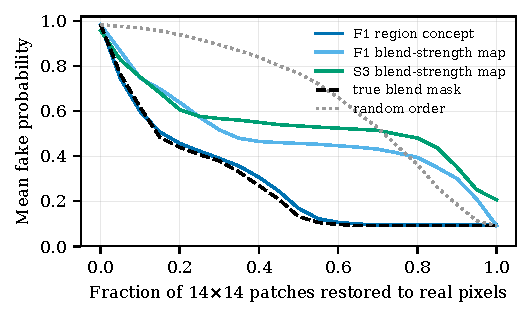
\includegraphics[width=\columnwidth]{fig_restoration.pdf}
\caption{Counterfactual restoration on 500 flagged SBI test images: mean fake probability as patches are restored to
the real source pixels in the order given by each map (F1 and S3 scored by their own model).}
\label{fig:restore}
\end{figure}

Fig.~\ref{fig:restore} and Table~\ref{tab:explain} show the result. The region concept reaches $R=0.281$, close to
the true mask (0.270), and after restoring 25\% of the patches the mean fake probability is 0.422 against 0.407 for
the mask and 0.907 for random order. The blend-strength maps of F1 (0.494) and S3 (0.544) also lie between the mask
and random order (0.663). Under a test that removes evidence by construction, the maps point at the pixels that
carry the decision, and the deletion failure above is a property of blur deletion. This conclusion holds for
self-blends, where the counterfactual is known; for real face swaps no real source frame exists, and the test does
not apply. Grad-CAM and rollout are omitted because B1 and C1 do not flag these images, so their curves start near
zero.

A related intervention on the same images switches off the top-scoring concept: the fake probability of F1 falls by
0.054 on average, against 0.011 for a randomly chosen other concept (S3: 0.022 vs.\ 0.005).

\begin{figure*}[t]
\centering
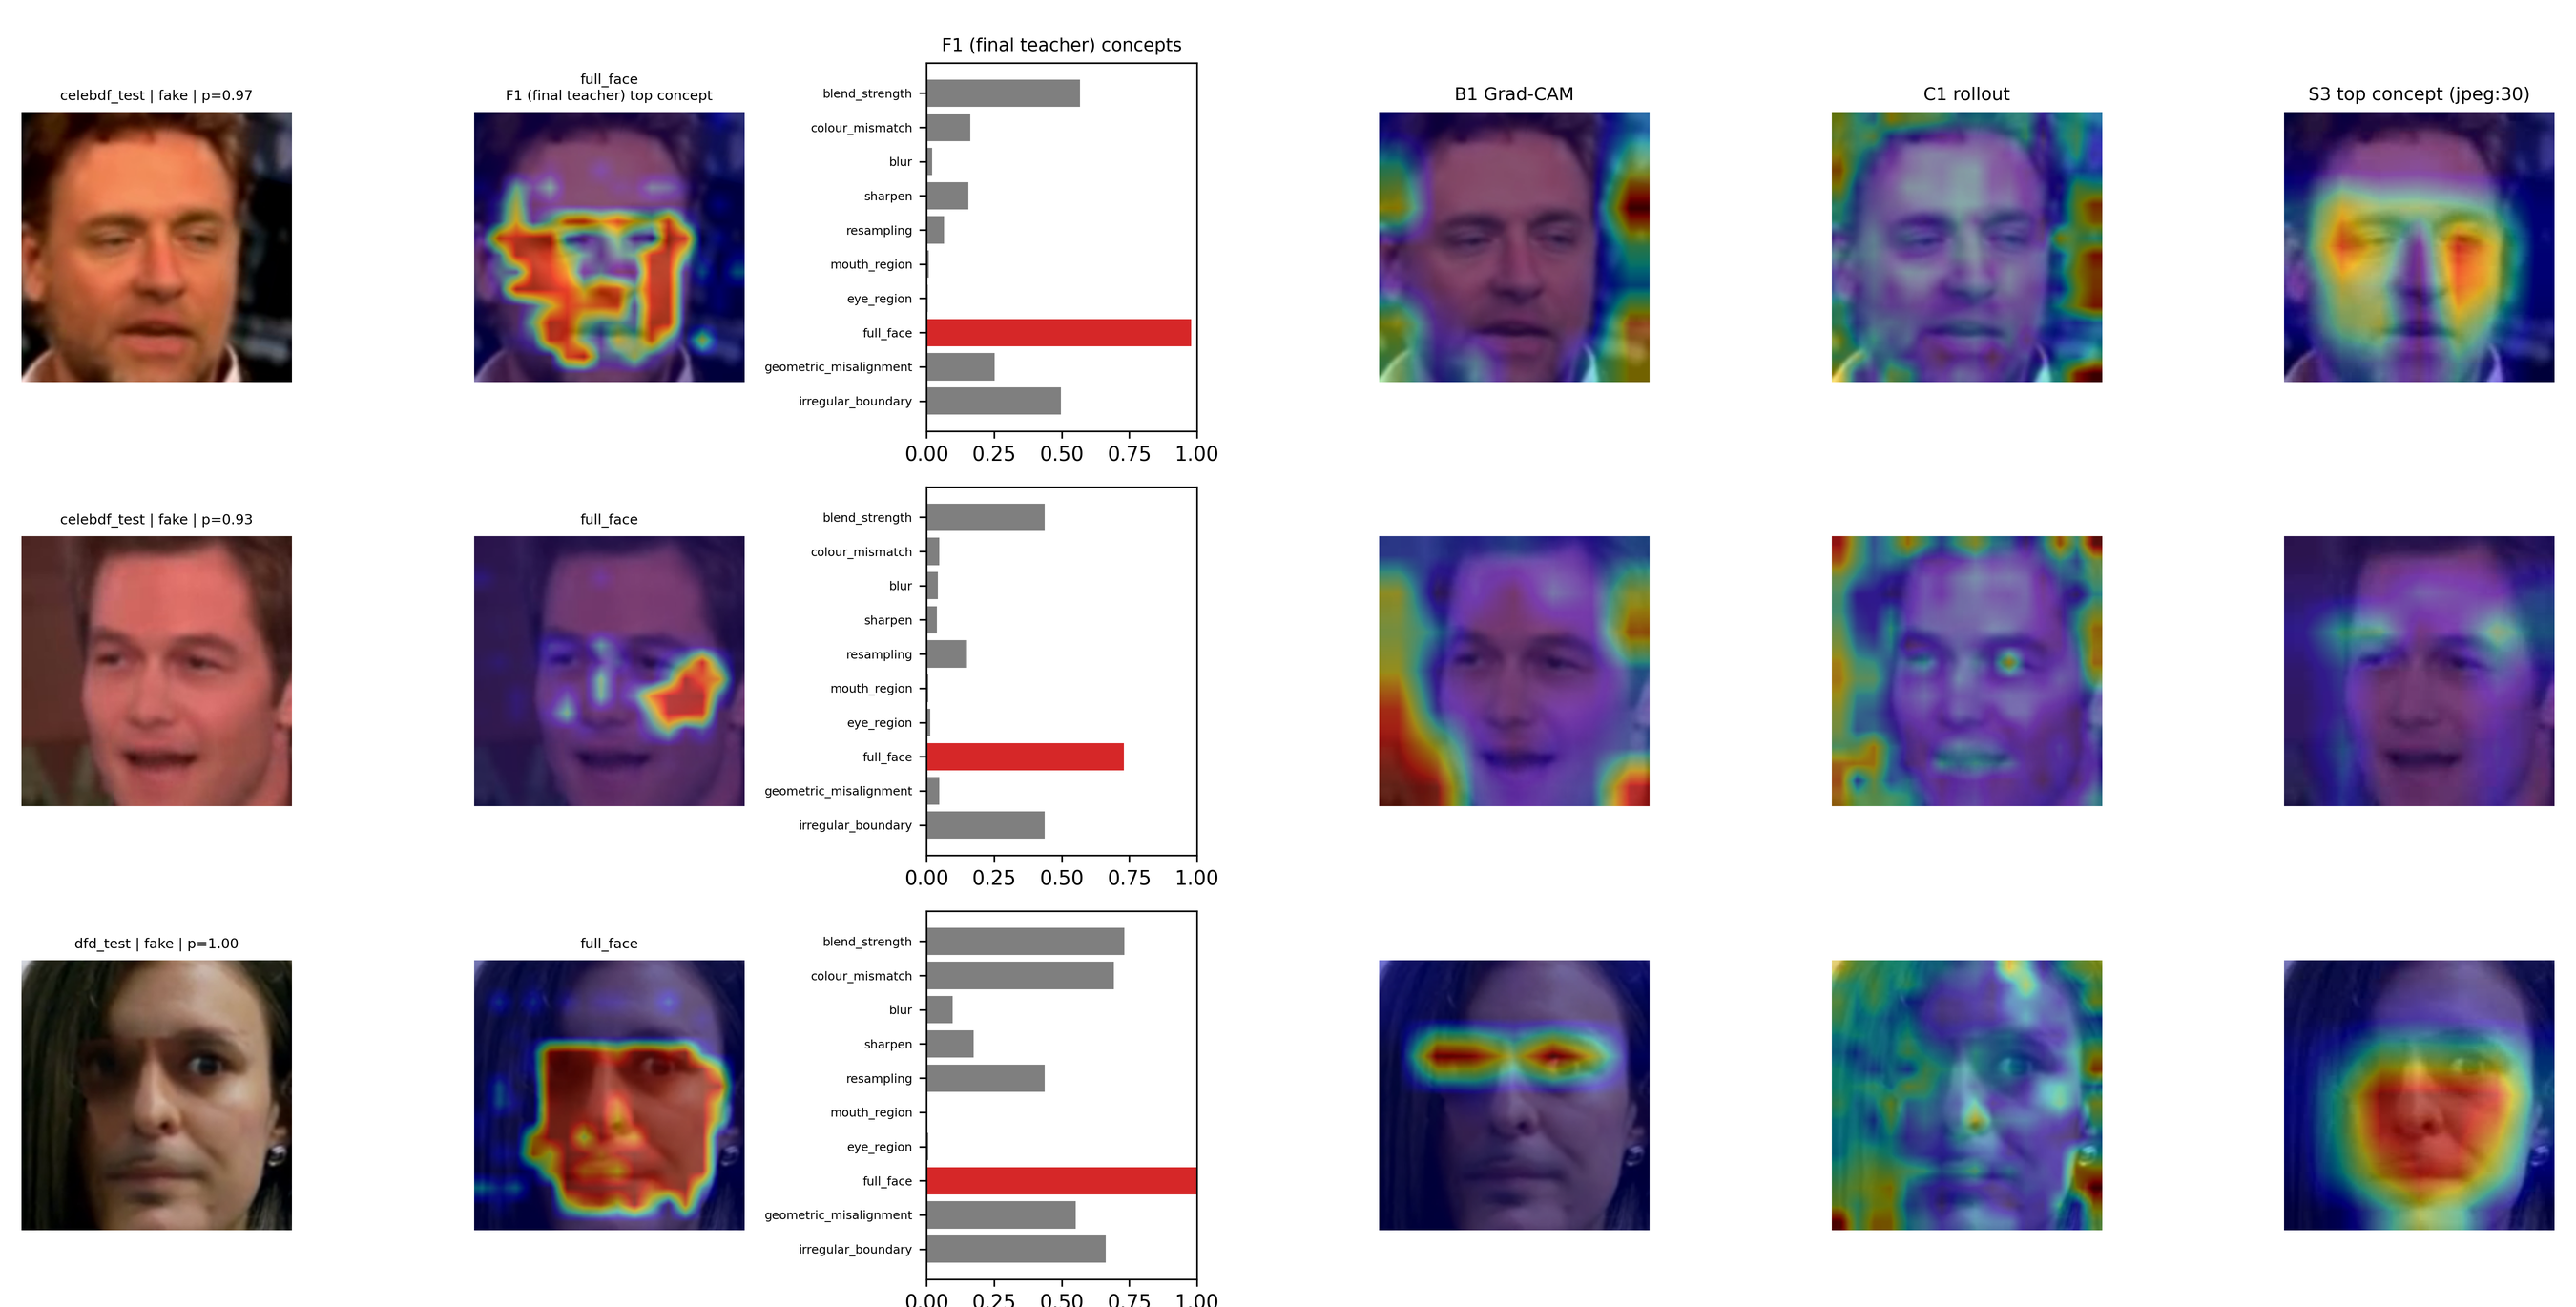
\includegraphics[width=\textwidth]{fig_explanations.png}
\caption{Explanations for three test fakes (two from Celeb-DF, one from DFD). From left: input with F1's fake
probability; F1's top concept map; F1's ten concept activations (top concept in red); Grad-CAM of B1; attention
rollout of C1; S3's top concept map on the JPEG-30 version of the frame.}
\label{fig:explain}
\end{figure*}

Fig.~\ref{fig:explain} shows three test fakes. In all three, full face is F1's top concept and its map covers the
swapped face region; the Grad-CAM and rollout maps of B1 and C1 concentrate on the background and image borders.

\subsection{Failure analysis on Celeb-DF}\label{sec:failure}
With the three F1 seeds averaged, Celeb-DF fakes are separated from Celeb-real videos with AUC 0.920 and from
YouTube-real videos with 0.832. Video sharpness (variance of the Laplacian over 8 crops) splits the test videos into
tertiles with AUC 0.888, 0.874 and 0.943 from least to most sharp. Of the 15 most confident errors at the validation
threshold, 13 are fakes with Laplacian variance between 5 and 14 that receive fake probabilities from 0.136 to
0.244, and two are YouTube-real videos scored 0.880 and 0.794. Blurry fakes and low-quality real uploads are the
two error modes; both are weak points of a decision driven by blending cues.

% =====================================================================================================
\section{Application}\label{sec:app}
The trained models run in a Gradio~\cite{gradio} web application. A careful mode uses F1 on a GPU and a quick mode
uses the ONNX student on a CPU; both sample frames from an uploaded video, detect and align faces, score each crop
and report the video score with the calibrated probability, the concept activations, the top concept map and a
switch-off control that applies Eq.~\eqref{eq:do} to chosen concepts. Because c10 is not learned
(Section~\ref{sec:interv}), its activation should be hidden from end users in a future version.

% =====================================================================================================
\section{Conclusion}\label{sec:conclusion}
Under source-video-disjoint splits, validation-only selection and three seeds with paired bootstrap intervals, a
CLIP ViT-L/14 detector whose logit passes through ten recipe-supervised concepts matches the clean cross-dataset AUC
of a CLIP-with-LoRA classifier (0.914 vs.\ 0.906, not statistically significant). The ablation assigns each
measured property to its source. Self-blended training data produces the JPEG robustness (0.789 to 0.898 at
quality 30) and most of the calibration gain on Celeb-DF. The concept bottleneck adds +0.009 to +0.016 cross AUC in
controlled comparisons and makes the decision inspectable: the ten concepts reproduce the model's AUC without the
residual, single-concept interventions show which cues decide individual videos, and the region maps remove
evidence as fast as the true blend mask in a counterfactual restoration test. Single-frame H.264 training raises AUC
at CRF 40 from 0.644 to 0.688, and the interventions show that this gain is carried by the concept path. Domain
alignment never helped, a larger training set helped more than any architecture change (0.944 vs.\ 0.878 on
Celeb-DF), and distilled students followed their training data rather than their teacher. The evaluation is limited to two face-swap test sets and a
reduced FF++ subset with three manipulation types; retraining on the full FF++ release is the next experiment.

Code, configurations, per-video predictions and the scripts that generate every table are available at
\url{https://github.com/pes1ug23cs178/CAPSTONE_PW_26_RJ_02}. The datasets are not redistributed.

\section*{Acknowledgment}
We thank the Department of Computer Science and Engineering, PES University, for compute resources.

\begin{thebibliography}{99}
\footnotesize
\bibitem{ffpp} A. Rössler, D. Cozzolino, L. Verdoliva, C. Riess, J. Thies, and M. Nießner, ``FaceForensics++: Learning to detect manipulated facial images,'' in \emph{Proc. IEEE/CVF Int. Conf. Computer Vision (ICCV)}, 2019, pp. 1--11.
\bibitem{dfd} N. Dufour and A. Gully, ``Contributing data to deepfake detection research,'' Google AI Blog, Sep. 24, 2019. [Online]. Available: \url{https://research.google/blog/contributing-data-to-deepfake-detection-research/}
\bibitem{celebdf} Y. Li, X. Yang, P. Sun, H. Qi, and S. Lyu, ``Celeb-DF: A large-scale challenging dataset for DeepFake forensics,'' in \emph{Proc. IEEE/CVF Conf. Computer Vision and Pattern Recognition (CVPR)}, 2020, pp. 3207--3216.
\bibitem{deepfakebench} Z. Yan, Y. Zhang, X. Yuan, S. Lyu, and B. Wu, ``DeepfakeBench: A comprehensive benchmark of deepfake detection,'' in \emph{Proc. Advances in Neural Information Processing Systems (NeurIPS), Datasets and Benchmarks Track}, 2023.
\bibitem{df40} Z. Yan, T. Yao, S. Chen, Y. Zhao, X. Fu, J. Zhu, D. Luo, C. Wang, S. Ding, Y. Wu, and L. Yuan, ``DF40: Toward next-generation deepfake detection,'' in \emph{Proc. Advances in Neural Information Processing Systems (NeurIPS), Datasets and Benchmarks Track}, 2024.
\bibitem{gradcam} R. R. Selvaraju, M. Cogswell, A. Das, R. Vedantam, D. Parikh, and D. Batra, ``Grad-CAM: Visual explanations from deep networks via gradient-based localization,'' in \emph{Proc. IEEE Int. Conf. Computer Vision (ICCV)}, 2017, pp. 618--626.
\bibitem{rollout} S. Abnar and W. Zuidema, ``Quantifying attention flow in transformers,'' in \emph{Proc. Annual Meeting of the Association for Computational Linguistics (ACL)}, 2020, pp. 4190--4197.
\bibitem{tsigos} K. Tsigos, E. Apostolidis, S. Baxevanakis, S. Papadopoulos, and V. Mezaris, ``Towards quantitative evaluation of explainable AI methods for deepfake detection,'' in \emph{Proc. ACM Int. Workshop on Multimedia AI against Disinformation (MAD '24)}, 2024, doi: 10.1145/3643491.3660292.
\bibitem{sbi} K. Shiohara and T. Yamasaki, ``Detecting deepfakes with self-blended images,'' in \emph{Proc. IEEE/CVF Conf. Computer Vision and Pattern Recognition (CVPR)}, 2022, pp. 18720--18729.
\bibitem{dfdc} B. Dolhansky, J. Bitton, B. Pflaum, J. Lu, R. Howes, M. Wang, and C. Canton Ferrer, ``The DeepFake Detection Challenge (DFDC) dataset,'' arXiv:2006.07397, 2020.
\bibitem{facexray} L. Li, J. Bao, T. Zhang, H. Yang, D. Chen, F. Wen, and B. Guo, ``Face X-ray for more general face forgery detection,'' in \emph{Proc. IEEE/CVF Conf. Computer Vision and Pattern Recognition (CVPR)}, 2020, pp. 5001--5010.
\bibitem{univfd} U. Ojha, Y. Li, and Y. J. Lee, ``Towards universal fake image detectors that generalize across generative models,'' in \emph{Proc. IEEE/CVF Conf. Computer Vision and Pattern Recognition (CVPR)}, 2023, pp. 24480--24489.
\bibitem{clip} A. Radford et al., ``Learning transferable visual models from natural language supervision,'' in \emph{Proc. Int. Conf. Machine Learning (ICML)}, 2021, pp. 8748--8763.
\bibitem{fa} X. Cui, Y. Li, A. Luo, J. Zhou, and J. Dong, ``Forensics Adapter: Adapting CLIP for generalizable face forgery detection,'' in \emph{Proc. IEEE/CVF Conf. Computer Vision and Pattern Recognition (CVPR)}, 2025, pp. 19207--19217.
\bibitem{effort} Z. Yan, J. Wang, P. Jin, K.-Y. Zhang, C. Liu, S. Chen, T. Yao, S. Ding, B. Wu, and L. Yuan, ``Orthogonal subspace decomposition for generalizable AI-generated image detection,'' in \emph{Proc. 42nd Int. Conf. Machine Learning (ICML)}, PMLR, vol. 267, 2025, pp. 70268--70288.
\bibitem{lnclip} A. Yermakov, J. Cech, J. Matas, and M. Fritz, ``Deepfake detection that generalizes across benchmarks,'' arXiv:2508.06248, 2025.
\bibitem{lora} E. J. Hu, Y. Shen, P. Wallis, Z. Allen-Zhu, Y. Li, S. Wang, L. Wang, and W. Chen, ``LoRA: Low-rank adaptation of large language models,'' in \emph{Proc. Int. Conf. Learning Representations (ICLR)}, 2022.
\bibitem{cbm} P. W. Koh, T. Nguyen, Y. S. Tang, S. Mussmann, E. Pierson, B. Kim, and P. Liang, ``Concept bottleneck models,'' in \emph{Proc. Int. Conf. Machine Learning (ICML)}, 2020, pp. 5338--5348.
\bibitem{whyfake} V. Vanian, A. Doumanoglou, and D. Zarpalas, ``Why fake? Unveiling the semantic vocabulary of deepfake detectors,'' in \emph{Proc. IEEE/CVF Conf. Computer Vision and Pattern Recognition Workshops (CVPRW)}, 2026, arXiv:2607.07216.
\bibitem{mansoor} N. Mansoor and A. I. Iliev, ``Explainable AI for DeepFake detection,'' \emph{Applied Sciences}, vol. 15, no. 2, Art. no. 725, Jan. 2025, doi: 10.3390/app15020725.
\bibitem{dfp2e} S. Tariq, S. S. Woo, P. Singh, I. Irmalasari, S. Gupta, and D. Gupta, ``From prediction to explanation: Multimodal, explainable, and interactive deepfake detection framework for non-expert users,'' in \emph{Proc. 33rd ACM Int. Conf. Multimedia (MM '25)}, 2025, doi: 10.1145/3746027.3755786.
\bibitem{laylens} A. Narang, P. Gupta, L. Su, and A. Dhall, ``LayLens: Improving deepfake understanding through simplified explanations,'' arXiv:2507.10066, 2025.
\bibitem{hinton} G. Hinton, O. Vinyals, and J. Dean, ``Distilling the knowledge in a neural network,'' arXiv:1503.02531, 2015.
\bibitem{ganin} Y. Ganin, E. Ustinova, H. Ajakan, P. Germain, H. Larochelle, F. Laviolette, M. Marchand, and V. Lempitsky, ``Domain-adversarial training of neural networks,'' \emph{J. Machine Learning Research}, vol. 17, no. 59, pp. 1--35, 2016.
\bibitem{mmd} A. Gretton, K. M. Borgwardt, M. J. Rasch, B. Schölkopf, and A. Smola, ``A kernel two-sample test,'' \emph{J. Machine Learning Research}, vol. 13, pp. 723--773, 2012.
\bibitem{irm} Z. Yin, J. Wang, Y. Xiao, H. Zhao, T. Li, W. Zhou, A. Liu, and X. Liu, ``Improving deepfake detection generalization by invariant risk minimization,'' \emph{IEEE Trans. Multimedia}, vol. 26, pp. 6785--6798, 2024, doi: 10.1109/TMM.2024.3355651.
\bibitem{fan} A. Bulat and G. Tzimiropoulos, ``How far are we from solving the 2D \& 3D face alignment problem? (and a dataset of 230,000 3D facial landmarks),'' in \emph{Proc. IEEE Int. Conf. Computer Vision (ICCV)}, 2017, pp. 1021--1030.
\bibitem{adamw} I. Loshchilov and F. Hutter, ``Decoupled weight decay regularization,'' in \emph{Proc. Int. Conf. Learning Representations (ICLR)}, 2019.
\bibitem{efficientnet} M. Tan and Q. V. Le, ``EfficientNet: Rethinking model scaling for convolutional neural networks,'' in \emph{Proc. Int. Conf. Machine Learning (ICML)}, 2019, pp. 6105--6114.
\bibitem{swin} Z. Liu, Y. Lin, Y. Cao, H. Hu, Y. Wei, Z. Zhang, S. Lin, and B. Guo, ``Swin Transformer: Hierarchical vision transformer using shifted windows,'' in \emph{Proc. IEEE/CVF Int. Conf. Computer Vision (ICCV)}, 2021, pp. 10012--10022.
\bibitem{guo} C. Guo, G. Pleiss, Y. Sun, and K. Q. Weinberger, ``On calibration of modern neural networks,'' in \emph{Proc. Int. Conf. Machine Learning (ICML)}, 2017, pp. 1321--1330.
\end{thebibliography}


\end{document}
